\chapter{Gestión del proyecto}

En este capítulo se detallan las metodologías de la gestión de proyectos que se han seguido en este trabajo presentes en el PMBOK\cite{pmbok}.


Las siguientes secciones describen el alcance del proyecto, la metodología de desarrollo, la planificación temporal, la gestión de la configuración, la gestión de costes y la gestión de riesgos.

%%%%%%%%%%%%%%%%%%%%%%%%%%%%%%%%%%%%%%%%%%%%%%%%%%%%%%%%%%%%%%%%%%%%%%%%%%%%%%%%%%%%%
%%%%%%%%%%%%%%%%%%%%%%%%%%%%%%%%%%%%%%%%%%%%%%%%%%%%%%%%%%%%%%%%%%%%%%%%%%%%%%%%%%%%%
%%%%%%%%%%%%%%%%%%%%%%%%%%%%%%%%%%%%%%%%%%%%%%%%%%%%%%%%%%%%%%%%%%%%%%%%%%%%%%%%%%%%%

\section{Alcance del proyecto}

Según el PMBOK\cite{pmbok} se trata del trabajo realizado para entregar un producto, servicio o resultado con las funciones y características especificadas. La línea base del proyecto, consistirá en el enunciado del alcance, la estructura de desglose de trabajo (EDT/WBS) y el diccionario EDT/WBS asociado.

\subsection{Enunciado del alcance}
Como promotora de la \textit{startup} Emozio, necesito una plataforma web que de viabilidad a mi modelo de negocio, el cual consiste en la asignación del psicólogo más adecuado para tratar la patología de un paciente. 


Como somos una \textit{startup} que ha surgido de forma reciente, todavía preciso validar y afianzar mi propuesta de valor para lanzarla al mercado. Por tanto, el requisito primordial es disponer de un producto mínimo viable que me permita mostrar esta propuesta a mi público objetivo.


Para desempeñar el producto mínimo viable necesito desarrollar una plataforma \textit{web} en la que pueda identificar una o varias posibles patologías en un determinado paciente. Una vez conocida la patología y el porcentaje de la misma en la caracterización del paciente, la plataforma le emparejará a un listado de psicólogos que podrían tratar una o varias de sus  patologías. Además, estos psicólogos podrán ser filtrados por distintos campos, como el precio, el seguro de salud, si se trata de una cita presencial u \textit{online}, entre otros. 


A su vez, debe permitir al paciente ponerse en contacto con el psicólogo del listado por el que desea ser atendido. Este mensaje de contacto, podrá visualizarlo el psicólogo a través de su bandeja de entrada. 


Cabe decir, que tanto psicólogos como pacientes podrán darse de alta en la plataforma y hacer uso de sus servicios, por lo que se necesitará una mínima gestión de usuarios. 


Para que el paciente pueda evaluar la cita recibida por el psicólogo, éste podrá dejar un comentario con una valoración en su perfil para que pueda ser compartido al resto de usuarios. De esta forma, se dará la transparencia necesaria al servicio de recomendación lo que nos valdrá de sello de calidad.

\subsection{Criterios de aceptación}
Las condiciones que deben cumplirse para que el proyecto sea aceptado son:

\begin{itemize}
\item Entrega en plazo de todos los entregables.
\item Realización de los requisitos esperados que tengan mayor prioridad.
\end{itemize}

\subsection{Entregables del proyecto}
Se deberá hacer entrega de:

\begin{itemize}
\item Tres copias en papel de la memoria, junto con el manual de instalación y los manuales de usuario
\item Una copia en soporte digital de:
	\begin{itemize}
		\item La memoria, junto con el manual de instalación y los manuales de usuario
		\item El código fuente
		\item El ejecutable
	\end{itemize}
\end{itemize}

\subsection{Exclusiones del proyecto}
Las exclusiones aplicadas al proyecto son:

\begin{itemize}
\item El mantenimiento y soporte de la plataforma una vez realizada la entrega.
\item Análisis de campo e investigación asociada al desarrollo del cuestionario científico de asignación.
\end{itemize}

\subsection{Restricciones del proyecto}
El alcance de este proyecto sólo abarcará el producto mínimo viable de lo que será la plataforma real de Emozio, y que servirá como punto de partida para la implementación de la misma. Su pretensión no se trata de realizar el desarrollo completo de la aplicación con todas sus características totalmente funcionales, sino realizar una primera aproximación a la misma.

\subsection{Supuestos del proyecto}
Asumimos que al tratarse de un producto mínimo viable, no se podrá estimar el crecimiento del sistema tanto a nivel de funcionalidades como en el contenido de la base de datos, por lo que no se podrá preveer cómo será la escalabilidad real del sistema.

\subsection{Estructura de descomposición de tareas (EDT/WBS) del proyecto}
La estructura de descomposición de tareas viene representada en la figura \ref{fig:edt}.

\begin{figure}[htbp] 
    \centering
    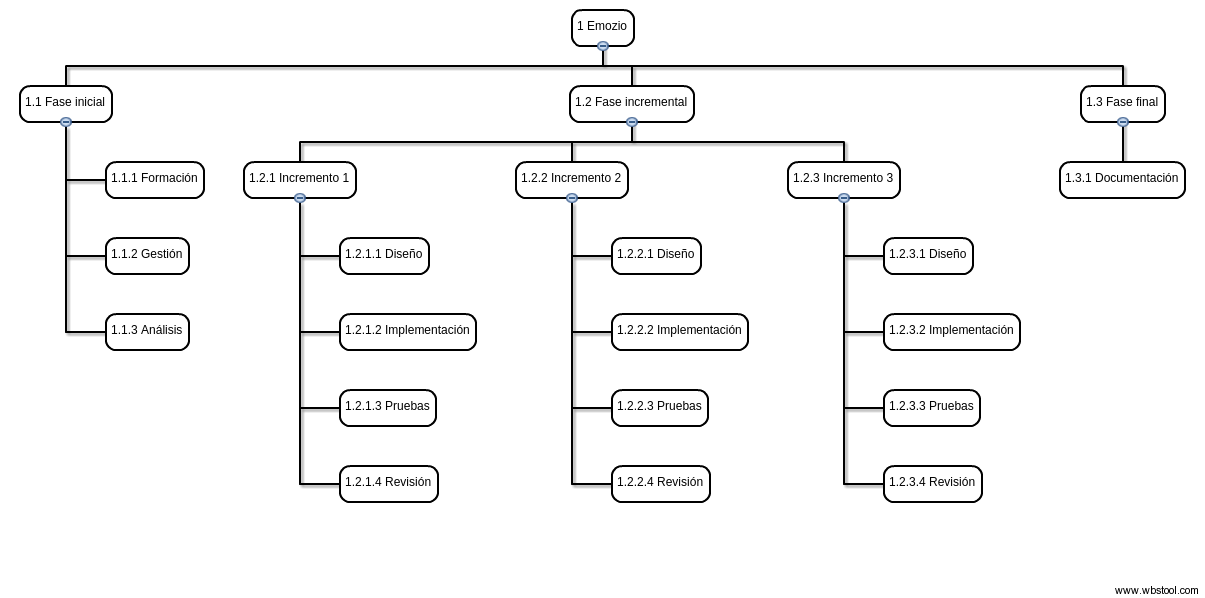
\includegraphics[width=1\textwidth]{figuras/edt_v1_en.png}
    \caption{Estructura de descomposición de tareas del proyecto}
    \label{fig:edt}
\end{figure}	

\subsubsection{Diccionario EDT/WBS}
El proyecto está dividido en tres fases: Inicial, incremental y final. Éstas se encuentran descritas en mayor detalle en la sección donde se detalla la metodología de desarrollo utilizada.

\begin{itemize}[label={}]
\item \textbf{Fase inicial}
Compuesta por la formación en las principales tecnologías utilizadas (\textit{Stack MEAN framework}), la elaboración de la gestión del proyecto y un primer análisis inicial del producto.
\item \textbf{Fase incremental}
Se encuentra dividida entre los tres incrementos que se van a realizar, cada uno con sus respectivas tareas: Diseño, implementación, pruebas y revisión.
\item \textbf{Fase final}
En ella se elaborará toda la documentación final del proyecto que se va a presentar: La memoria, el manual de instalación y el manual de usuario.
\end{itemize} 

%%%%%%%%%%%%%%%%%%%%%%%%%%%%%%%%%%%%%%%%%%%%%%%%%%%%%%%%%%%%%%%%%%%%%%%%%%%%%%%%%%%%%
%%%%%%%%%%%%%%%%%%%%%%%%%%%%%%%%%%%%%%%%%%%%%%%%%%%%%%%%%%%%%%%%%%%%%%%%%%%%%%%%%%%%%
%%%%%%%%%%%%%%%%%%%%%%%%%%%%%%%%%%%%%%%%%%%%%%%%%%%%%%%%%%%%%%%%%%%%%%%%%%%%%%%%%%%%%

\section{Metodología de desarrollo}
Una metodología de desarrollo de software en ingeniería de software es un marco de trabajo usado para estructurar, planificar y controlar el proceso de desarrollo en sistemas de información.


Según Pressman\cite{pressman}, cualquier proceso del software ágil se caracteriza por la forma en la que aborda cierto número de suposiciones clave acerca de la mayoría de proyectos de software:

\begin{itemize}
\item Es difícil predecir que requerimientos de software persistirán y cuales cambiarán o pronosticar como cambiaron las prioridades del cliente a medida que avanza el proyecto.
\item En muchos tipos de software el diseño y la construcción de ejecutarse en forma simultánea de modo que los modelos de diseño se prueban a medida que se crean.
\item El análisis, el diseño, la construcción y las pruebas no son tan predecibles como nos gustaría.
\end{itemize} 


Las principales motivaciones para utilizar este tipo de metodología se trataban de:

\begin{itemize}
\item Inicialmente, se desconocía mucha información: Como el algoritmo que se iba a utilizar para el emparejamiento, como la caracterización de los pacientes y psicólogos, como la información que era necesario almacenar en la base datos\dots
\item Existía la posibilidad de que el psicólogo experto, mi principal \textit{stakeholder} el cuál me iba a proporcionar el \textit{feedback} e información necesaria del sistema, me pidiese cambios repentinos al descubrir nueva información relevante a cerca del emparejamiento.
\item Por otra parte, sí se tenían claro los subsistemas que se requerían dentro de la plataforma.
\item Como se trata de un proyecto que surge de un estado del arte, necesitábamos gran margen para introducir cambios y poder integrarlos.
\item La inexperiencia en las tecnologías utilizadas podrían suponer que hubiese continuos cambios en el diseño y el código de la plataforma.
\end{itemize}


Por tanto, se requería un proceso adaptativo e incremental, donde en cada incremento se desarrollase uno de los subsistemas identificados en nuestra plataforma.


En este tipo de procesos, deben entregarse incrementos de software (prototipos ejecutables o porciones de un sistema) en periodos cortos de tiempo. Este enfoque iterativo permite que el cliente evalúe de forma regular el incremento de software, dé la retroalimentación necesaria e influya en las adaptaciones del proceso que se realicen para aprovechar esa retroalimentación.


Las fases que se van a realizar en este proyecto son:
\begin{enumerate}
\item \textbf{Fase Inicial:} Conlleva la gestión de proyecto, la formación y un primer análisis inicial de lo que sería la plataforma.
\item \textbf{Fase incremental:} En esta fase se realizarán los tres incrementos.
\item \textbf{Fase final:} Se realizará la documentación del proyecto.
\end{enumerate}

\subsubsection{Fase incremental}
En esta sección se describirán con mayor detalle en qué consisten los tres incrementos del proceso. Donde cada uno de ellos tendrá sus propias fases de diseño, implementación, pruebas y revisión. \newline

\textbf{Incremento 1}\newline


El primer incremento se realizará justo después de la fase inicial, y se corresponde con el subsistema del cuestionario de emparejamiento paciente-psicólogo.


Según la planificación temporal descrita en la gestión de tiempos, se prevé que el incremento 1 comience el día 9 de noviembre y finalice el 6 de diciembre. Esta previsión tiene en cuenta que es el primer contacto directo con las tecnologías utilizadas por lo que es predecible que se trabaje de forma más pautada y se produzcan muchos ensayo-error. Además de que en él se implementa la complejidad algorítmica relacionada con el emparejamiento.\newline


\textbf{Incremento 2}\newline


Tras finalizar el primer incremento, se procede a realizar este segundo que se corresponde con el subsistema de gestión de usuarios.


Según la planificación prevista, estará comprendido entre el 7 de diciembre y el 20 de diciembre.\newline


\textbf{Incremento 3}\newline


El último incremento es el subsistema de comunicación. 


Siguiendo la planificación temporal realizada, durará desde el 21 de diciembre hasta el 3 de enero.


A lo largo de esta memoria cada tarea realizada, estará definida dentro del contexto del incremento en el cual se realiza.

%%%%%%%%%%%%%%%%%%%%%%%%%%%%%%%%%%%%%%%%%%%%%%%%%%%%%%%%%%%%%%%%%%%%%%%%%%%%%%%%%%%%%
%%%%%%%%%%%%%%%%%%%%%%%%%%%%%%%%%%%%%%%%%%%%%%%%%%%%%%%%%%%%%%%%%%%%%%%%%%%%%%%%%%%%%
%%%%%%%%%%%%%%%%%%%%%%%%%%%%%%%%%%%%%%%%%%%%%%%%%%%%%%%%%%%%%%%%%%%%%%%%%%%%%%%%%%%%%

\section{Planificación temporal}
La previsión temporal del presente proyecto estaba comprendido entre el 16 de octubre de 2017 y el 21 de enero de 2018, con un trabajo de seis horas diarias. La estimación temporal en tareas, y la asignación de las mismas a los recursos, se puede observar en el diagrama de Gantt \ref{fig:gantt}.

\begin{landscape}

\begin{figure}[htbp] 
    \centering
    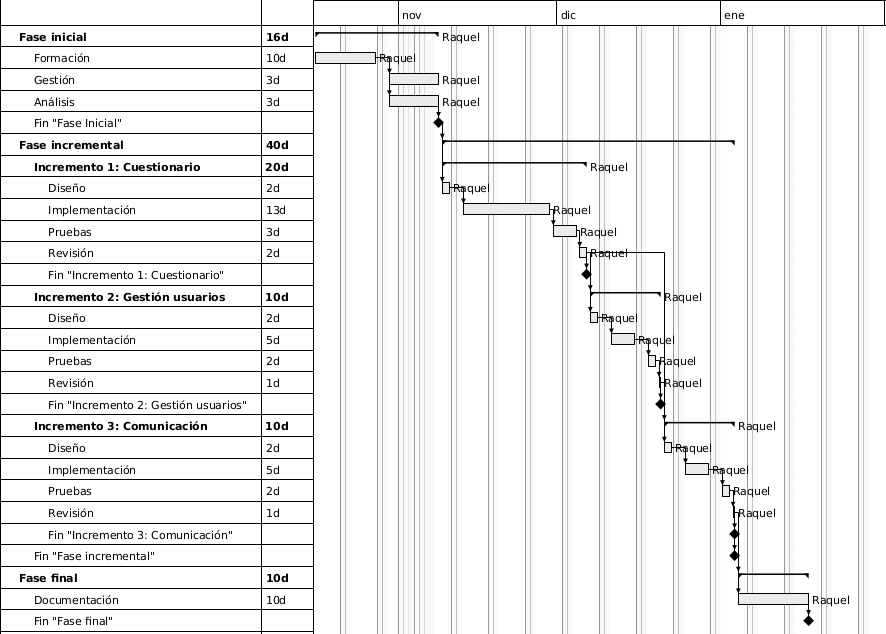
\includegraphics[height=\textwidth,keepaspectratio]{figuras/gantt_v2_en.png}
    \caption{Diagrama de Gantt}
    \label{fig:gantt}
\end{figure}	

\end{landscape}

%%%%%%%%%%%%%%%%%%%%%%%%%%%%%%%%%%%%%%%%%%%%%%%%%%%%%%%%%%%%%%%%%%%%%%%%%%%%%%%%%%%%%
%%%%%%%%%%%%%%%%%%%%%%%%%%%%%%%%%%%%%%%%%%%%%%%%%%%%%%%%%%%%%%%%%%%%%%%%%%%%%%%%%%%%%
%%%%%%%%%%%%%%%%%%%%%%%%%%%%%%%%%%%%%%%%%%%%%%%%%%%%%%%%%%%%%%%%%%%%%%%%%%%%%%%%%%%%%

\section{Gestión de la configuración}
La gestión de la configuración del software es un conjunto de actividades diseñadas para administrar el cambio mediante la identificación de los productos de trabajo con potencial de cambio, las relaciones entre ellos, la definición de mecanismos para administrar diferentes versiones de los mismos y el control de los cambios impuestos, así como la auditoría y reporte de los cambios realizados\cite{pressman}.

\subsection{Línea base}
El IEEE (IEEE Std. No. 610.12-1990) indica que una especificación o producto que se revisó formalmente y con el que se estuvo de acuerdo, servirá como base para un mayor desarrollo y que cambia sólo a través de procedimientos de control de cambio formal.


Las líneas base de nuestro proyecto son fundamentalmente el enunciado del alcance del proyecto, los requisitos \textit{software}, el diseño y el código del anterior incremento (si existe).

\subsubsection{Creación de líneas base}
Como nuestro proyecto se desarrolla de manera incremental, la línea base del segundo incremento, será tanto el enunciado del alcance del proyecto, los requisitos software asociados a dicho incremento y finalmente, el código resultado del incremento 1. De forma análoga sería para el caso del incremento 3, que tendría como línea base adicional el código resultado del incremento 2.

\subsection{Repositorio para la gestión de la configuración}
Un repositorio es el conjunto de mecanismos y estructuras de datos que permiten administrar el cambio de forma efectiva, asegurando la integridad, posibilidad de compartir e integrar datos. Para lograr estas capacidades, el repositorio se define como un metamodelo que determina cómo se almacena la información en el repositorio, cómo pueden acceder las herramientas a los datos, cuán bien puede mantenerse la seguridad e integridad de los datos y cuán fácilmente puede extenderse el modelo existente para alojar nuevas necesidades\cite{pressman}.

\subsubsection{Repositorio escogido}
Este proyecto se encuentra almacenado en un repositorio GitHub que es una plataforma de desarrollo colaborativo de software para alojar proyectos usando el sistema de control de versiones Git\cite{github}. Git nos permitirá tener una copia del repositorio del proyecto en local y otra en remoto. El proyecto en local sufrirá constantes modificaciones, que una vez validadas, se guardarán en el remoto.

\subsubsection{Metamodelo}
La estructura de información que se encuentra en el repositorio viene definida en la tabla \ref{tab_metamodelo}.

\begin{table}[htpb]
\centering
\begin{tabularx}{\textwidth}{|l|l|X|}
\hline
\multicolumn{2}{|c|}{\textbf{Carpeta}}                     & \multicolumn{1}{c|}{\textbf{Descripción del contenido}}                                                                             \\ \hline
\multicolumn{2}{|X|}{em\_diagramas}               & Contiene el archivo de StarUML que contiene todos los diagramas del proyecto: Casos de uso, modelo de datos, patrón MVC... \\ \hline
\multirow{8}{*}{em\_memoria} & em\_analisis       & Contiene todos los archivos referentes al análisis.                                                                        \\ \cline{2-3} 
                             & em\_anexos         & Contiene todos los anexos de la memoria del proyecto.                                                                      \\ \cline{2-3} 
                             & em\_diseño         & Contiene todos los archivos referentes al diseño.                                                                          \\ \cline{2-3} 
                             & em\_implem         & Contiene todos los archivos referentes a la implementación.                                                                          \\ \cline{2-3} 
                             & em\_gest\_proy     & Contiene todos los archivos referentes a la gestión del proyecto.                                                          \\ \cline{2-3} 
                             & em\_introducción   & Contiene la introducción de la memoria del proyecto.                                                                       \\ \cline{2-3} 
                             & em\_memoria\_final & Se trata del documento en LaTeX que contiene la memoria a entregar.                                                        \\ \cline{2-3} 
                             & em\_plan\_pruebas  & Contiene todos los archivos referentes al plan de pruebas.                                                                 \\ \hline
\multicolumn{2}{|X|}{em\_mockup}                  & Contiene el mockup hecho con Pencil de la plataforma web.                                                                  \\ \hline
\multicolumn{2}{|X|}{em\_web}                     & Contiene todos los archivos que constituyen el código fuente de la plataforma web.                                         \\ \hline
\end{tabularx}
\caption{Metamodelo}
\label{tab_metamodelo}
\end{table}

Dentro de cada carpeta o subcarpeta, los archivos aparecen con un nombre descriptivo. Por ejemplo, en la subcarpeta de \texttt{em\_memoria} llamada \texttt{em\_gest\_proy} se encuentra \texttt{gest\_costes.odt} que es el archivo correspondiente a la subsección de costes de la sección de gestión del proyecto que habrá en la memoria final.

\subsection{Sistema de gestión de la configuración}
La estructura del repositorio está distribuida del siguiente modo:

\begin{enumerate}
\item \textbf{Master}
Contendrá la última versión validada del código fuente, es decir, tras pasar las pruebas del incremento 1, contendrá el código fuente del incremento 1, y así, sucesivamente.
\item \textbf{Branches}
	\begin{itemize}
	\item \textbf{memoria\_branch}
	Contendrá los commits de las distintas versiones de la memoria del proyecto.
	\item \textbf{diagrama\_branch}
	Contendrá los commits de las distintas versiones de los diagramas de la plataforma.
	\item \textbf{mockup\_branch}
	Contendrá los commits de las distintas versiones del mockup de la plataforma.
	\item \textbf{cuestionario\_branch, usuarios\_branch y contacto\_branch}
	Contendrán respectivamente, los \textit{commits} del código fuente asociado a los incrementos 1, 2 y 3.
	Antes de comenzar un incremento, se crea una \textit{branch} de \textit{master} y se implementan las funcionalidades pertenecientes a ese incremento. Una vez realizada su fase de pruebas, se hará un \textit{merge} de esa \textit{branch} con el \textit{master}, y posteriormente, se elimina.
	\end{itemize}
\end{enumerate}


%%%%%%%%%%%%%%%%%%%%%%%%%%%%%%%%%%%%%%%%%%%%%%%%%%%%%%%%%%%%%%%%%%%%%%%%%%%%%%%%%%%%%
%%%%%%%%%%%%%%%%%%%%%%%%%%%%%%%%%%%%%%%%%%%%%%%%%%%%%%%%%%%%%%%%%%%%%%%%%%%%%%%%%%%%%
%%%%%%%%%%%%%%%%%%%%%%%%%%%%%%%%%%%%%%%%%%%%%%%%%%%%%%%%%%%%%%%%%%%%%%%%%%%%%%%%%%%%%

\section{Gestión de costes}

En esta sección nos centraremos en los costes que engloba el proyecto. Para poder llevar a cabo la estimación de los costes, los cálculos se realizarán por estimación paramétrica\cite{pmbok}, que tiene en cuenta los datos históricos relevantes y otras variables, para calcular una estimación del coste del trabajo del proyecto.


Las estimaciones son evaluaciones cuantitativas de los costes probables que se requieren para completar el trabajo del proyecto, que involucran a todos los recursos incluídos, entre otros, el trabajo directo, los materiales, el equipamiento y la tecnología de la información. En nuestras estimaciones, no se tendrán en cuenta aquellos costes que sean indirectos.


A continuación, se encuentran dispuestas por categorías las diferentes estimaciones de costes.


\subsection{Costes del personal}
Para calcular los costes asociados a los recursos humanos del proyecto, se tendrá como referencia al estudio realizado por Vitae Consultores que ha dado como resultado la Guía Salarial del Sector TI en Galicia 2015-2016\cite{vitae}.


Como datos principales para nuestros cálculos, el estudio muestra que una analista programadora que tenga entre 0 o 2 años de experiencia, cobra de media 1600 \euro brutos.


Para realizar los cálculos referentes a los recursos humanos, se ha empleado la calculadora de contratos para la Gestión de actividad I+D de la Oficina de Investigación y Tecnología de la USC\cite{calculadoracontratos}.


Los datos introducidos para hacer los cálculos fueron los siguientes:
\begin{itemize}
\item \textbf{Salario bruto mensual:} 16000 \euro
\item \textbf{Periodo de contrato:} 16/10/2017 a 21/01/2018
\item \textbf{Número de pagas:} 14
\item \textbf{Tipo de contrato:} Obra y servicio
\item \textbf{Jornada laboral:} Tiempo completo
\item \textbf{Horas semanales:} 37,5
\item \textbf{Categoría cotización:} Ingeniera – Licenciada – Grado; Técnico administrativo
\end{itemize}


Los resultados obtenidos son los que aparecen en la tabla\ref{fig:calc_cont}.


\begin{table}[htpb]
\centering
\begin{tabularx}{\textwidth}{|X|X|X|X|X|}
\hline
\multirow{2}{*}{\textbf{Mes}}      & 1            & 2              & 3              & 4          \\ \cline{2-5} 
                                   & Octubre 2017 & Noviembre 2017 & Diciembre 2017 & Enero 2018 \\ \hline
\textbf{Días trabajados}           & 16           & 30             & 31             & 21         \\ \hline
\textbf{Retribución Bruta Mensual} & 1.600,00 €   & 1.600,00 €     & 1.600,00 €     & 1.600,00 € \\ \hline
\textbf{Base de Cotización}        & 963,44 €     & 1.866,67 €     & 1.866,67 €     & 1.264,52 € \\ \hline
\textbf{Salario Bruto}             & 825,81 €     & 1.600,00 €     & 1.600,00 €     & 1.083,87 € \\ \hline
\textbf{Pagas Extras}              & 0,00 €       & 0,00 €         & 402,19 €       & 457,15 €   \\ \hline
\textbf{Cota Patronal}             & 309,27 €     & 599,20 €       & 599,20 €       & 405,91 €   \\ \hline
\textbf{Liquidación}               & 32,28 €      & 60,53 €        & 62,55 €        & 42,37 €    \\ \hline
\end{tabularx}
\caption{Calculadora de contratos}
\label{fig:calc_cont}
\end{table}


El resumen anual sería el que se muestra en la tabla\ref{fig:res_anual}.

\begin{table}[htpb]
\centering
\begin{tabular}{|l|l|l|l|l|}
\hline
\textbf{}                 & 2017       & 2018       & \multicolumn{2}{l|}{\multirow{3}{*}{}} \\ \cline{1-3}
\textbf{Bruto}            & 4.025,81 € & 1.083,87 € & \multicolumn{2}{l|}{}                  \\ \cline{1-3}
\textbf{Pagas extras}     & 402,19 €   & 457,15 €   & \multicolumn{2}{l|}{}                  \\ \hline
\textbf{Liquidación}      & -          & 197,73 €   & \textbf{Liquidación}    &              \\ \hline
\textbf{Coste contrato}   & 4.428,00 € & 1.738,75 € & 197,73 €                & 6.166,75 €   \\ \hline
\textbf{Seguridad Social} & 1.507,67 € & 405,91 €   &                         & 1.913,58 €   \\ \hline
\textbf{TOTAL}            & 5.935,67 € & 2.144,66 € &                         & 8.080,33 €   \\ \hline
\end{tabular}
\caption{Resumen anual}
\label{fig:res_anual}
\end{table}


\subsection{Costes de \textit{hardware}}
Para calcular los costes asociados al \textit{hardware} empleado en el proyecto primero vemos los dispositivos que empleamos en el mismo. Después, su coste asociado, y por último, calculamos su depreciación debido al tiempo que tienen y a las horas de trabajo que lo hemos empleado.


El ordenador portátil empleado para el proyecto ha sido un Sony Vaio Modelo SVF1521N6EW con tres años de vida. El cálculo de uso medio del portátil es de 300 horas de trabajo al año. Según este cálculo, el tiempo de vida útil del mismo, su costo de compra, y el trabajo del proyecto hemos generado la siguiente tabla\ref{fig:coste_hw}.


\begin{table}[htpb]
\centering
\begin{tabular}{|l|l|}
\hline
\textbf{Coste de compra}             & 640,00 \euro     \\ \hline
\textbf{Vida útil}                   & 4 años       \\ \hline
\textbf{Antigüedad}                  & 3 años       \\ \hline
\textbf{Horas de uso en el proyecto} & 400 h        \\ \hline
\textbf{Depreciación}                & 160,00 \euro/año \\ \hline
\textbf{Valor Actual}                & 160,00 \euro     \\ \hline
\textbf{Coste asociado al hardware}  & 120,00 \euro     \\ \hline
\end{tabular}
\caption{Coste del \textit{hardware}}
\label{fig:coste_hw}
\end{table}


\subsection{Costes del \textit{software} y formación}
Como podemos ver en el apartado de herramientas utilizadas, todas las empleadas son de código libre, debido a este factor no corresponden coste alguno para el proyecto en lo relativo a su uso para la realización del mismo.


Estas tecnologías usadas no incrementan coste por su simple uso, sin embargo, para la correcta y eficiente realización del proyecto con las tecnologías escogidas se ha seguido un curso que sí ha supuesto un coste a tener en cuenta.


Se ha realizado un curso \textit{online} para el correcto aprendizaje de las tecnologías utilizadas que se pueden ver en el apartado del mismo nombre. Este curso se ha realizado durante los meses del proyecto y sus costes asociados se pueden ver en la siguiente tabla\ref{fig:coste_sw}.


\begin{table}[htpb]
\centering
\begin{tabular}{|l|l|}
\hline
\textbf{Meses cursados} & \textbf{Coste por mes} \\ \hline
Octubre                 & 25,00 \euro                \\ \hline
Noviembre               & 25,00 \euro                \\ \hline
Diciembre               & 25,00 \euro                \\ \hline
Enero                   & 25,00 \euro                \\ \hline
\textbf{Coste total}    & 100,00 \euro               \\ \hline
\end{tabular}
\caption{Costes de formación relacionados con el \textit{software}}
\label{fig:coste_sw}
\end{table}


\subsection{Costes indirectos}
En lo referido a los costes indirectos del proyecto se incluyen aquellos paralelos a la realización del proyecto, que, sin tener directa relación con el contenido del trabajo, sí son necesarios para poder llevarlos a cabo. Los costes indirectos identificados son los siguientes:
\begin{itemize}
\item Gasto de electricidad
\item Gasto de desplazamiento
\item Gasto de tarifas telefónicas de datos
\end{itemize}


Estos gastos indirectos no se pueden añadir en su totalidad a los costes totales del proyecto debido a que su uso no ha sido centrado únicamente en la realización de nuestro proyecto.


Para calcular por tanto estos costes indirectos se refleja un porcentaje de los costes de personal y activos anteriores del 10 \%. El resultado se puede ver en la tabla\ref{fig:coste_indirecto}.


\begin{table}[htpb]
\centering
\begin{tabular}{|l|l|}
\hline
\textbf{Costes del personal}            & 8.080,33 \euro \\ \hline
\textbf{Costes de Hardware}             & 120 \euro      \\ \hline
\textbf{Costes de Software y formación} & 100 \euro      \\ \hline
\textbf{Porcentaje}                     & 10\%       \\ \hline
\textbf{Costes indirectos}              & 830,03 \euro   \\ \hline
\end{tabular}
\caption{Costes indirectos}
\label{fig:coste_indirecto}
\end{table}


\subsection{Resumen de los costes totales}
En la tabla\ref{fig:coste_total}, vemos el desglose y suma total de cada uno de los costes asociados al proyecto.


\begin{table}[htpb]
\centering
\begin{tabular}{|l|l|}
\hline
\textbf{Costes del personal}            & 8.080,33 \euro \\ \hline
\textbf{Costes de Hardware}             & 120 \euro      \\ \hline
\textbf{Costes de Software y formación} & 100 \euro      \\ \hline
\textbf{Costes indirectos}              & 830,03 \euro   \\ \hline
\textbf{TOTAL}                          & 9.130,36 \euro \\ \hline
\end{tabular}
\caption{Resumen de los costes totales}
\label{fig:coste_total}
\end{table}





%%%%%%%%%%%%%%%%%%%%%%%%%%%%%%%%%%%%%%%%%%%%%%%%%%%%%%%%%%%%%%%%%%%%%%%%%%%%%%%%%%%%%
%%%%%%%%%%%%%%%%%%%%%%%%%%%%%%%%%%%%%%%%%%%%%%%%%%%%%%%%%%%%%%%%%%%%%%%%%%%%%%%%%%%%%
%%%%%%%%%%%%%%%%%%%%%%%%%%%%%%%%%%%%%%%%%%%%%%%%%%%%%%%%%%%%%%%%%%%%%%%%%%%%%%%%%%%%%

\section{Gestión de riesgos}

\subsection{Plan de gestión de riesgos}
El riesgo de un proyecto es un evento o condición incierta que, de producirse, tiene un efecto positivo o negativo en uno o más de los objetivos del proyecto. Éste, puede tener una o más causas, y de materializarse, uno o más impactos\cite{pmbok}.


Para poder prevenir estas consecuencias, se debe llevar un registro de los posibles riesgos que pueden acontecer. Así, una vez identificados y analizados, podemos planificar las respuestas para los mismos.


Para poder definir la probabilidad e impacto de la materialización de un riesgo, se deben definir las escalas correspondientes a los mismos. Para poder medir la probabilidad e impacto que puede tener un riesgo se han creado las tablas \ref{tab_probabilidad} y \ref{tab_impacto}.


La \textbf{probabilidad} representa la expectativa de ocurrencia real del riesgo, y el \textbf{impacto}, representa el efecto que la ocurrencia del riesgo tendría en el desarrollo del proyecto, en términos de coste, esfuerzo o duración total del mismo. 

\begin{table}[htpb]
\centering
\begin{tabular}{|l|l|}
\hline
\rowcolor[gray]{0.9}\multicolumn{2}{|c|}{\textbf{Valoración del impacto}}                                                  \\ \hline
\multicolumn{1}{|c|}{\textbf{Repercusión en Plazo / Esfuerzo / Costes}} & \multicolumn{1}{c|}{\textbf{Impacto}} \\ \hline
\textgreater= 20\%                                             & Alto                         \\ \hline
Entre 10\% y 20 \%                                             & Medio                        \\ \hline
\textless= 10\%                                                & Bajo                         \\ \hline
\end{tabular}
\caption{Valoración del impacto}
\label{tab_impacto}
\end{table}

\begin{table}[htpb]
\centering
\begin{tabular}{|l|l|}
\hline
\rowcolor[gray]{0.9}\multicolumn{2}{|c|}{\textbf{Valoración de la probabilidad}} \\ \hline
\multicolumn{1}{|c|}{\textbf{Ocurrencia del Riesgo}}             & \multicolumn{1}{c|}{\textbf{Probabilidad}}  \\ \hline
\textgreater= 80\% (casi segura)  & Alta          \\ \hline
Entre 30\% y 80\% (muy probable)  & Media         \\ \hline
\textless= 30\% (poco probable)   & Baja         \\ \hline
\end{tabular}
\caption{Valoración de la probabilidad}
\label{tab_probabilidad}
\end{table}

Si vinculamos la probabilidad de ocurrencia de cada riesgo con su impacto sobre los objetivos del proyecto en caso de que ocurra dicho riesgo, podemos obtener la matriz que representa el nivel de exposición al riesgo (dado por el producto del impacto por la probabilidad). Esta matriz \ref{tab_riesgo} determinará la gestión de los riesgos del proyecto.

\begin{table}[htpb]
\centering
\begin{tabular}{|l|l|l|l|l|}
\hline
\rowcolor[gray]{0.9}\multicolumn{5}{|c|}{\textbf{Nivel de exposición al riesgo}}                         \\ \hline
\multicolumn{2}{|l|}{\multirow{2}{*}{}} & \multicolumn{3}{c|}{\textbf{Probabilidad}} \\ \cline{3-5} 
\multicolumn{2}{|l|}{}                  & Alta      & Media     & Baja      \\ \hline
\multirow{3}{*}{\textbf{Impacto}}     & Alto     & Alto      & Alto      & Medio     \\ \cline{2-5} 
                             & Medio    & Alto      & Medio     & Bajo      \\ \cline{2-5} 
                             & Bajo     & Medio     & Bajo      & Bajo      \\ \hline
\end{tabular}
\caption{Nivel de exposición al riesgo}
\label{tab_riesgo}
\end{table}

\subsection{Identificación de riesgos}
Tras identificar los riesgos por medio  de revisión de la documentación, tormenta de ideas y análisis de supuestos, se procede a la elaboración del siguiente registro de riesgos \ref{tab_reg_riesgos}.

\begin{table}[htpb]
\centering
\begin{tabularx}{\textwidth}{|l|X|X|}
\hline
\rowcolor[gray]{0.9}\multicolumn{1}{|c|}{\textbf{Identificador}} & \multicolumn{1}{c|}{\textbf{Nombre}}                        & \multicolumn{1}{c|}{\textbf{Descripción}}                                                                                                                                                              \\ \hline
RSG-001                             & Práctica deficiente de la gestión de proyectos     & Se produce una práctica deficiente en la gestión de proyectos debido a la inexperiencia.                                                                                                      \\ \hline
RSG-002                             & Dependencia de participantes externos              & Existe dependencia de participantes externos fuera del ámbito de control directo del proyecto como el tutor que guía el proyecto o el experto psicólogo.                                      \\ \hline
RSG-003                             & Falta de experiencia en las tecnologías utilizadas & La inexperiencia en las tecnologías utilizadas puede repercutir en la planificación prevista del proyecto.                                                                                    \\ \hline
RSG-004                             & Pérdida de información                             & Se puede producir la pérdida de información debido a un mal guardado de los datos en el respositorio.                                                                                         \\ \hline
RSG-005                             & Retraso en la planificación temporal               & Acontece un retraso en la planificación temporal prevista debido a causas externas como enfermedad o asuntos personales.                                                                      \\ \hline
RSG-006                             & Caída de la red proveedora de Internet             & Una caída de la red proveedora de Internet puede causar retrasos en la planificación o pérdida deinformación.                                                                                 \\ \hline
RSG-007                             & Fallo de suministro eléctrico                      & Un fallo del suministro eléctrico  puede causar retrasos en la planificación o pérdida deinformación.                                                                                         \\ \hline
RSG-008                             & Ataques maliciosos en el equipo de trabajo         & Un ataque malicioso en el equipo de trabajo puede significar que existe una brecha de seguridad en el sistema por lo que existe un posible robado de datos o incluso pérdidas de información. \\ \hline
\end{tabularx}
\caption{Registro de riesgos}
\label{tab_reg_riesgos}
\end{table}

\subsection{Análisis cualitativo de riesgos}
Mediante el análisis cualitativo de los riesgos podemos evaluar la prioridad de los riesgos identificados a través de la probabilidad relativa de ocurrencia, del impacto correspondiente sobre los objetivos del proyecto si los riesgos llegasen a presentarse. Esta evaluación \ref{tab_eval_riesgos} refleja la actitud que existe frente a los riesgos. 

\begin{table}[htpb]
\centering
\begin{tabularx}{\textwidth}{|l|X|l|l|l|}
\hline
\rowcolor[gray]{0.9}\multicolumn{1}{|c|}{\textbf{Identificador}} & \multicolumn{1}{c|}{\textbf{Nombre}}                        & \multicolumn{1}{c|}{\textbf{Probabilidad}} & \multicolumn{1}{c|}{\textbf{Impacto}} & \multicolumn{1}{c|}{\textbf{Exposición}} \\ \hline
RSG-001                             & Práctica deficiente de la gestión de proyectos     & Media                             & Alto                         & Alto                            \\ \hline
RSG-002                             & Dependencia de participantes externos              & Alta                              & Medio                        & Alto                            \\ \hline
RSG-003                             & Falta de experiencia en las tecnologías utilizadas & Alta                              & Alto                         & Alto                            \\ \hline
RSG-004                             & Pérdida de información                             & Baja                              & Alto                         & Medio                           \\ \hline
RSG-005                             & Retraso en la planificación temporal               & Baja                              & Medio                        & Bajo                            \\ \hline
RSG-006                             & Caída de la red proveedora de Internet             & Baja                              & Alto                         & Medio                           \\ \hline
RSG-007                             & Fallo de suministro eléctrico                      & Baja                              & Alto                         & Medio                           \\ \hline
RSG-008                             & Ataques maliciosos en el equipo de trabajo         & Baja                              & Alto                         & Medio                           \\ \hline
\end{tabularx}
\caption{Evaluación de los riesgos}
\label{tab_eval_riesgos}
\end{table}

La matriz de exposición de los riesgos \ref{tab_mat_exp_riesgo} da a conocer las prioridades de acción en el caso de que se materializasen los riesgos.

\begin{table}[htpb]
\centering
\begin{tabular}{|c|c|l|l|l|}
\hline
\multicolumn{2}{|l|}{\multirow{2}{*}{}} & \multicolumn{3}{c|}{\textbf{Probabilidad}}                                                                                                      \\ \cline{3-5} 
\multicolumn{2}{|l|}{}                  & \multicolumn{1}{c|}{Alta} & \multicolumn{1}{c|}{Media} & \multicolumn{1}{c|}{Baja}                                                     \\ \hline
\multirow{3}{*}{Impacto}     & Alto     & RSG-003                   & RSG-001                    & \begin{tabular}[c]{@{}l@{}}RSG-004\\ RSG-006\\ RSG-007\\ RSG-008\end{tabular} \\ \cline{2-5} 
                             & Medio    & RSG-002                   &                            & RSG-005                                                                       \\ \cline{2-5} 
                             & Bajo     &                           &                            &                                                                               \\ \hline
\end{tabular}
\caption{Matriz de exposición de los riesgos}
\label{tab_mat_exp_riesgo}
\end{table}

\subsection{Plan de respuesta a los riesgos}
Con la planificación de respuesta a los riesgos se busca desarrollar opciones y acciones para mejorar las oportunidades y reducir las amenazas a los objetivos del proyecto. Las respuestas a los riesgos deben adecuarse a la importancia del riesgo, ser rentables con relación al desafía a cumplir,  realistas dentro del contexto del proyecto y a cargo de una persona responsable \cite{pmbok}.


Debido a que sólo existe una persona a cargo del proyecto, ésta será la responsable de acatar las medidas oportunas.


\begin{table}[htpb]
\centering
\begin{tabularx}{\textwidth}{|l|X|}
\hline
\rowcolor[gray]{0.9}\textbf{RSG-001}              & \textbf{Práctica deficiente de la gestión de proyectos} \\ \hline
Acción de prevención & Mitigar. Se asegurará que la persona encargada de la gestión de proyectos se forme específicamente en dicho ámbito. \\ \hline
Indicador            & La persona encargada de la gestión no efectúa adecuadamente los procesos a seguir.                                  \\ \hline
Acción de corrección & Se dedicarán más horas de trabajo a la gestión de proyectos.                                                        \\ \hline
\end{tabularx}
\caption{Plan de respuesta RSG-001}
%\label{my-label}
\end{table}


\begin{table}[htpb]
\centering
\begin{tabularx}{\textwidth}{|l|X|}
\hline
\rowcolor[gray]{0.9}\textbf{RSG-002}              & \textbf{Dependencia de participantes externos}                                                                                                                                                                  \\ \hline
Estrategia & Minimizar. Debido a la imprevisión que supone estar a expensas de otro \textit{stakeholder} del proyecto se plantea mover las reuniones agendadas. \\ \hline
Indicador            & Ausencia o falta de respuesta por parte de un \textit{stakeholder}.                                                                                                                                             \\ \hline
Acción de corrección & Se procederá a abordar las distintas tareas de forma ficticia o en último recurso se obviarán.                                                                                                        \\ \hline
\end{tabularx}
\caption{Plan de respuesta RSG-002}
%\label{my-label}
\end{table}


\begin{table}[htpb]
\centering
\begin{tabularx}{\textwidth}{|l|X|}
\hline
\rowcolor[gray]{0.9}\textbf{RSG-003}              & \textbf{Falta de experiencia en las tecnologías utilizadas}                                                                \\ \hline
Estrategia & Mitigar. Se formará al trabajador en las tecnologías utilizadas antes de comenzar con el desarrollo del proyecto. \\ \hline
Indicador            & El trabajador desconoce cómo implementar determinada funcionalidad                                                \\ \hline
Acción de corrección & Se pausará por un determinado tiempo el desarrollo y se estudiará lo necesario para poder continuar.              \\ \hline
\end{tabularx}
\caption{Plan de respuesta RSG-003}
%\label{my-label}
\end{table}


\begin{table}[htpb]
\centering
\begin{tabularx}{\textwidth}{|l|X|}
\hline
\rowcolor[gray]{0.9}\textbf{RSG-004}              & \textbf{Pérdida de información}                                                                                                  \\ \hline
Estrategia & Acción preventiva. Se harán volcados del trabajo realizado en el repositorio de forma periódica de al menos dos días de trabajo.  \\ \hline
Indicador            & Los últimos cambios efectuados no están reflejados en los archivos de trabajo ni en la última versión del repositorio. \\ \hline
Acción de corrección & Se repartirá el número de horas de trabajo correspondiente a esa parte durante el próximo periodo de la planificación.  \\ \hline
\end{tabularx}
\caption{Plan de respuesta RSG-004}
%\label{my-label}
\end{table}


\begin{table}[htpb]
\centering
\begin{tabularx}{\textwidth}{|l|X|}
\hline
\rowcolor[gray]{0.9}\textbf{RSG-005}              & \textbf{Retraso en la planificación temporal}                                                                                                                                                     \\ \hline
Estrategia & Minimizar. Debido a que se puede producir un retraso en la planificación temporal por causas ajenas al proyecto, se recuperarán las horas perdidas reubicándolas en la planificación temporal. \\ \hline
Indicador            & Surge una enfermedad o un asunto personal.                                                                                                                                               \\ \hline
Acción de corrección & Se reubicará la carga de trabajo prevista y que no haya sido realizada a lo largo del periodo que vaya a continuación.                                                                   \\ \hline
\end{tabularx}
\caption{Plan de respuesta RSG-005}
%\label{my-label}
\end{table}


\begin{table}[htpb]
\centering
\begin{tabularx}{\textwidth}{|l|X|}
\hline
\rowcolor[gray]{0.9}\textbf{RSG-006}              & \textbf{Caída de la red proveedora de Internet}                                                                                                                                                                 \\ \hline
Estrategia & Mitigar. Se dispondrá de una red alternativa a la que usamos de forma habitual.                                                                                                                        \\ \hline
Indicador            & Falla la conexión a Internet o no se encuentra la red.                                                                                                                                                 \\ \hline
Acción de corrección & Se procederá a buscar una red alternativa. Por ejemplo, en el caso de estar trabajando con la conexión WiFi y que ésta sufra una caída, proceder a conectarnos a la red móvil del \textit{smartphone} personal. \\ \hline
\end{tabularx}
\caption{Plan de respuesta RSG-006}
%\label{my-label}
\end{table}


\begin{table}[htpb]
\centering
\begin{tabularx}{\textwidth}{|l|X|}
\hline
\rowcolor[gray]{0.9}\textbf{RSG-007}              & \textbf{Fallo de suministro eléctrico                                                                                                                                } \\ \hline
Estrategia & Minimizar. Se procede a hacer copias de seguridad de forma periódica. Si el fallo de suministro eléctrico causa una pérdida del trabajo realizado, se retoma el trabajo a partir de la última copia de seguridad existente. \\ \hline
Indicador            & El ordenador se queda sin suministro eléctrico de forma repentina tras una subida de tensión.                                                                 \\ \hline
Acción de corrección & Se rehará el trabajo a partir de la última versión guardada.                                                                                                  \\ \hline
\end{tabularx}
\caption{Plan de respuesta RSG-007}
%\label{my-label}
\end{table}


\begin{table}[htpb]
\centering
\begin{tabularx}{\textwidth}{|l|X|}
\hline
\rowcolor[gray]{0.9}\textbf{RSG-008}              & \textbf{Ataques maliciosos en el equipo de trabajo}                                                                                                                                                              \\ \hline
Estrategia & Evitar. No descargar recursos de fuentes no fiables, no utilizar el ordenador de trabajo como ordenador personal, no dejar la sesión abierta en caso de ausencia y que ésta posea contraseña de acceso. \\ \hline
Indicador            & Fallos desconocidos hasta el momento en el sistema, pérdida de información, comportamiento sospechosos del funcionamiento del ordenador...                                                              \\ \hline
Acción de corrección & Se hará un formateo del sistema y se recuperarán los últimos cambios, de ser afectados, de la última versión del repositorio.                                                                           \\ \hline
\end{tabularx}
\caption{Plan de respuesta RSG-008}
%\label{my-label}
\end{table}






